%*********************************************************************************
%-----------------------------------Comments--------------------------------------
%*********************************************************************************

% For more information regading fonts, visit:
% http://tex.loria.fr/general/new/fntguide.html

%*********************************************************************************
%---------------------------Beginning of the template-----------------------------
%*********************************************************************************

\documentclass[a4paper,12pt]{article}

%*********************************************************************************
%-----------------------------------Packages--------------------------------------
%*********************************************************************************

	\usepackage{graphicx} 	% To include pictures
	\usepackage{subfigure} 	% To have the funtionality of multiple pictures per figure
	\usepackage{pstricks} 	% To use the functionality of a powerful drawing tool and position some pictures correctly
 	\usepackage{epsfig} 	% Extra package for .eps graphics usage
 	\usepackage{pst-grad} 	% For gradients
 	\usepackage{pst-plot} 	% For axes
	\usepackage{amsmath} 	% Extra math symbols There are a lot of ams packages
	\usepackage{fancyhdr} 	% To use fancy headers and footers --- requires for most proffesional docs
	\usepackage{watermark} 	% To include a figure in the backround - the frontpage for example
	\usepackage{enumerate} 	% To enumerate your items in a list with any style
	\usepackage[colorlinks=true, linkcolor=blue, citecolor=red, urlcolor=blue]{hyperref} % hyperlinks etc, must be the last package in the package list.
	\usepackage{epstopdf}
	\usepackage{float} 		% To use [H] when spacing figures
	
	\usepackage{enumitem}		% Better list spacing
	\setlist{nolistsep}			% No spacing in lists
	\usepackage{pdfpages} 		% Include pdf docs
	\usepackage{setspace}		% Line spacing
	\usepackage[bottom]{footmisc} 	% Force footnotes to the bottom of the page
	\usepackage{booktabs} 		% Better tables with toprule
	\usepackage{xcolor} 		% For colour manipulation
	\usepackage{anyfontsize}	% For flexible fontsize
	\usepackage{bold-extra} 	% For font case in pspicture
	\usepackage{pgfplotstable}	% To create tables from csv files
	\usepackage[explicit]{titlesec}

    %Tables
    \usepackage{multirow}
    \usepackage{booktabs}
    \usepackage{color}
    \usepackage{colortbl}
    
    %Fonts
    \usepackage{helvet}
    
%*********************************************************************************
%---------------------------------Custom Packages---------------------------------
%*********************************************************************************

%	\usepackage{./lib/sectioning} 	% Section Styles
%	\input{./lib/macros.tex}		% Collection of custom commands

%*********************************************************************************
%-------------------------------------Defines-------------------------------------
%*********************************************************************************

%Color
\definecolor{NWU_PURPLE}{rgb}{0.44, 0.16, 0.48}

%Font
%\renewcommand{\rmdefault}{phv}

%*********************************************************************************
%-------------------------------Titles and Authors--------------------------------
%*********************************************************************************

\title	{
\fontfamily{phv} \Huge \textcolor{NWU_PURPLE}{FACULTY OF ENGINEERING}\\
\vspace{2.5 cm} 
\textbf{REII 414}\\
\huge \textbf{Practical:\\E-Learing Platform}\vspace{0.8 cm}
}

\author{ \Large \bf by: \\ \Large\bf
\begin{tabular}{l  r}
Jacques Beukes & 26028107\\
Dewald Krynauw & ********\\
\end{tabular}\\\\
Submitted in pursuit of the degree\\\\
\bf BACHELOR OF ENGINEERING\\\\
\bf In\\\\
\bf COMPUTER AND ELECTRONIC ENGINEERING\\\\
\bf North-West-University Potchefstroom Campus
\\
\\
\\
\hspace*{-9 cm} % if you want the following info on the left hand side of the page 
\begin{tabular}{l} \\
	Supervisor: Mr. A. Alberts\\
	Potchefstroom \\
	2018 				
\end{tabular}
}

\date{}

%*********************************************************************************
%-------------------------Page styles & headers & footers-------------------------
%*********************************************************************************
	
\parskip=6pt 			% the size of the space between paragraphs
\setlength{\parindent}{0pt} % to indent the paragraph
\pagestyle{fancy}
\headheight=15pt 		% Have enough space so that the header can fit without warnings
\headwidth=6.7in 		% The width of the header 
\textwidth=6.6in 		% The width of the text
\oddsidemargin=0in 		% The margin indent on odd pagenumbers
\evensidemargin=0in 	% The margin indent on even pagenumbers

\rhead{
\begin{pspicture}(0,0)(0,0)

\includegraphics[scale=0.4]{./images/NWU_header.eps} 
\end{pspicture}
}
\chead{} % center header
\lhead{\textbf{\textsf{\footnotesize FACULTY OF ENGINEERING}}}

\rfoot{\thepage} 
\cfoot{\today} 
\lfoot{REII 414 Practical} 

\renewcommand{\headrulewidth}{1pt}
\renewcommand{\footrulewidth}{1pt} 	% To increase the header or footer line size

\numberwithin{equation}{section} % Number figures and equations according to the section working in
\numberwithin{figure}{section}


%*********************************************************************************
%----------------------------Beginning of the document----------------------------
%*********************************************************************************

\begin{document}

%*********************************************************************************
%-----------------------------------Front Page------------------------------------
%*********************************************************************************
\pagenumbering{roman} 	% First pages are number in Roman numerals

\enlargethispage{10\baselineskip} % To change the height of this front page for the title

\thiswatermark{
\begin{pspicture}(2.75,25)(2.75,25)
    
\includegraphics[scale=1]{./images/NWU_front_page.png} 
\end{pspicture}
} 

\maketitle

\thispagestyle{empty} 	% This page should not have header or footers

\pagebreak
%*********************************************************************************
%------------------------------------Abstract-------------------------------------
%*********************************************************************************

%\renewcommand{\abstractname}{\Large Abstract}
%\begin{abstract}
%\begin{large}
%******
%\end{large}
%\end{abstract}

\pagebreak

%*********************************************************************************
%-------------------------------Table of contents---------------------------------
%*********************************************************************************

%\renewcommand{\contentsname}{Table of Contents}
\tableofcontents 


%*********************************************************************************
%-------------------------------------Lists---------------------------------------
%*********************************************************************************

\section*{\Large{Abbreviations}}
%\begin{center}
%\begin{tabular}{l l}
%PWM & Pulse Width Modulation\\
%RPM & Revolutions Per Minute\\
%PI & Proportional-Integral\\
%\end{tabular}
%\end{center}

\listoffigures

\listoftables

\pagebreak
%*********************************************************************************
%-------------------------------------Body----------------------------------------
%*********************************************************************************

\pagenumbering{arabic}

\section{Introduction}



\section{Background}

\section{Database}

\section{Front-end}

\subsection{Login and Register Interface}
\begin{figure}[H]
\centering
\fbox{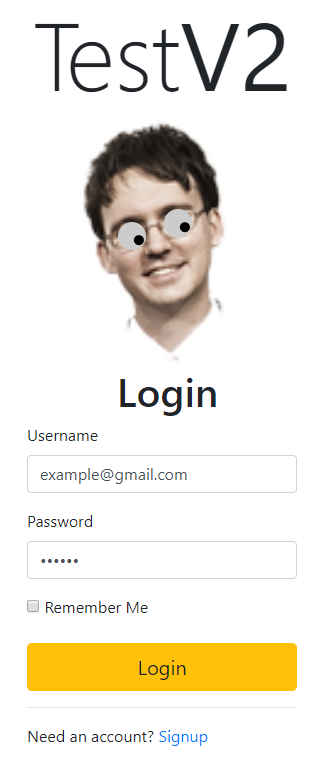
\includegraphics[scale = 0.6]{./images/login.png}}
\caption{Login page}
\label{login}
\end{figure}

\begin{figure}[H]
\centering
\fbox{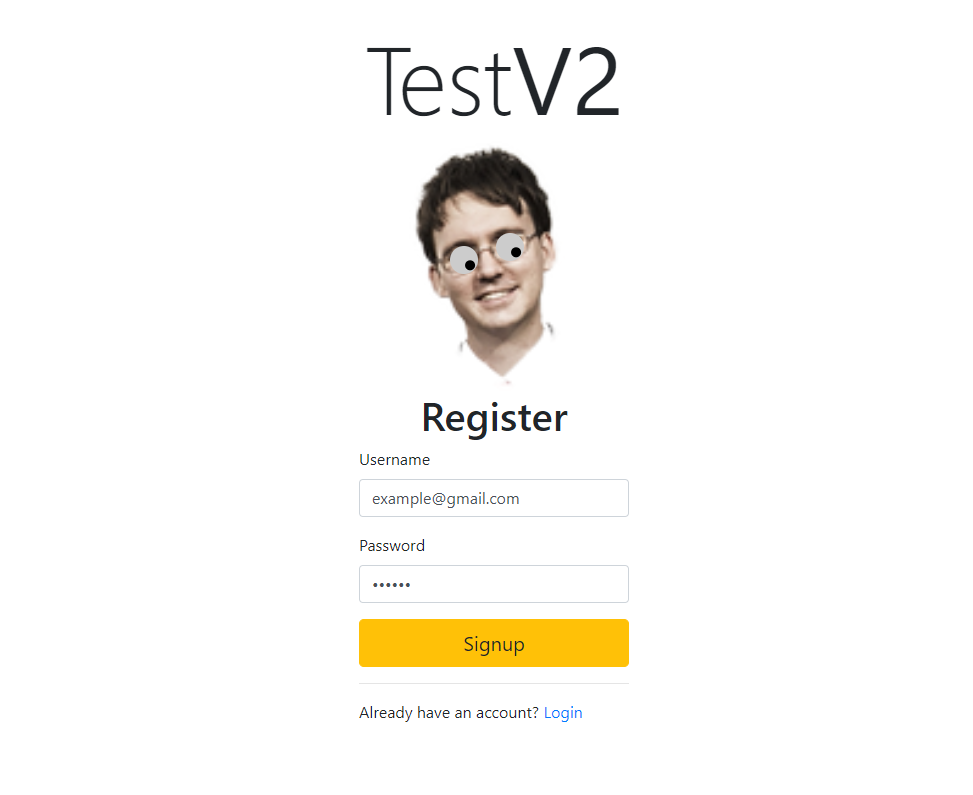
\includegraphics[scale = 0.6]{./images/register.png}}
\caption{Register page}
\label{register}
\end{figure}



\subsection{Lecturer Interface}

\begin{figure}[H]
\centering
\fbox{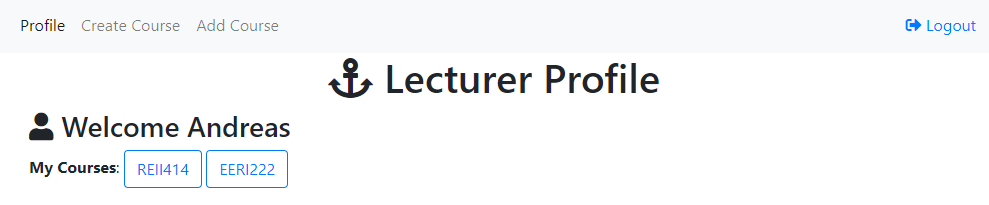
\includegraphics[scale = 0.6]{./images/lecturerProfile.png}}
\caption{Lecturer profile page}
\label{lecturerProfile}
\end{figure}

\newcommand{\picScale}{0.55}
\newcommand{\minipageWidth}{0.46\textwidth}

\begin{figure}[H]
\minipage[t]{\minipageWidth}
	\centering
	\fbox{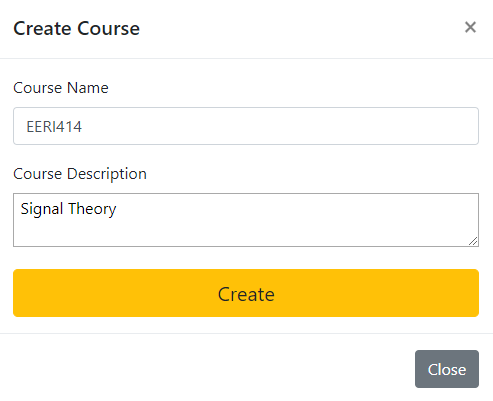
\includegraphics[scale = \picScale]{./images/createCourse.png}}
	\vspace{-0.2cm}
	\caption{Page for creating a course}
	\label{createCourse}
\endminipage\hfill
\minipage[t]{\minipageWidth}
	\centering
	\fbox{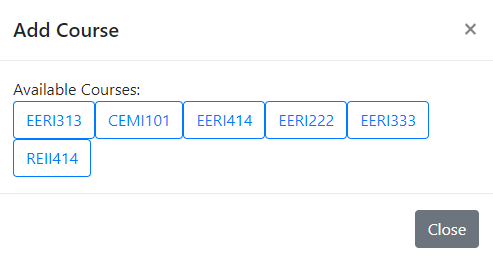
\includegraphics[scale = \picScale]{./images/addCourse.png}}
	\vspace{-0.2cm}
	\caption{Page for adding a course}
	\label{addCourse}
\endminipage
\end{figure}

\begin{figure}[H]
\centering
\fbox{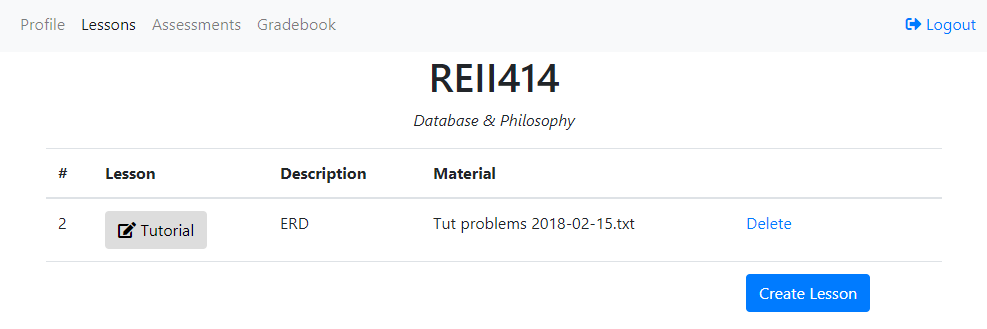
\includegraphics[scale = 0.6]{./images/lecturerLessons.png}}
\caption{Lecturer lessons page}
\label{lecturerLessons}
\end{figure}

\begin{figure}[H]
\centering
\fbox{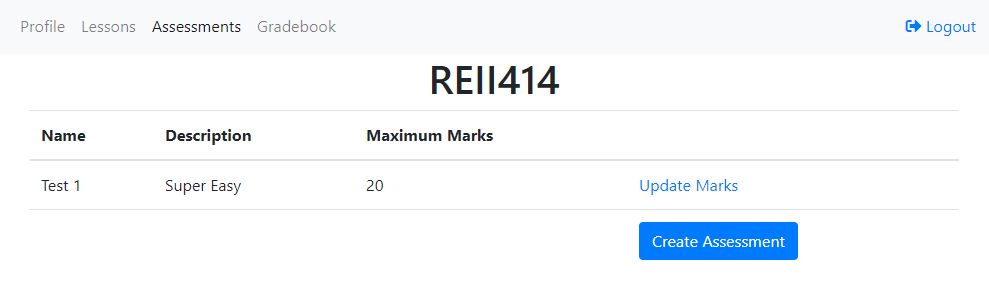
\includegraphics[scale = 0.6]{./images/lecturerAssessments.png}}
\caption{Lecturer assessments page}
\label{lecturerAssessments}
\end{figure}

\begin{figure}[H]
\centering
\fbox{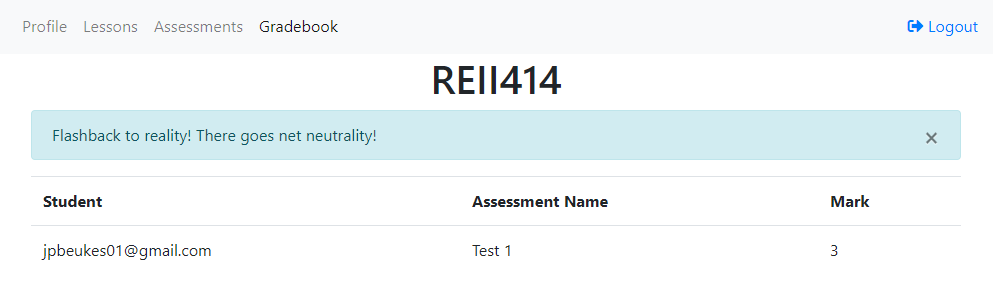
\includegraphics[scale = 0.6]{./images/lecturerGradebook.png}}
\caption{Lecturer gradebook page}
\label{lecturerGradebook}
\end{figure}

\begin{figure}[H]
\minipage[t]{\minipageWidth}
	\centering
	\fbox{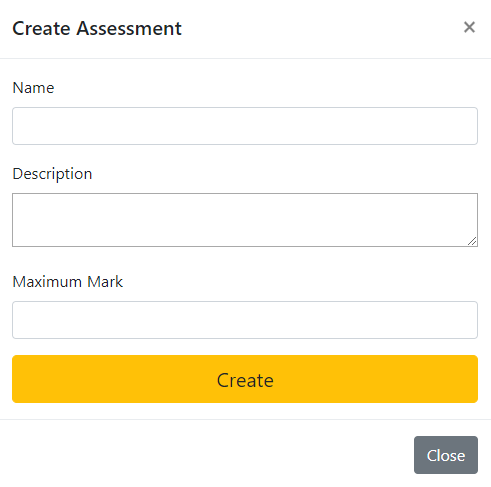
\includegraphics[scale = \picScale]{./images/lecturerCreateAssessment.png}}
	\vspace{-0.2cm}
	\caption{Creating assessments page}
	\label{lecturerCreateAssessment}
\endminipage\hfill
\minipage[t]{\minipageWidth}
	\centering
	\fbox{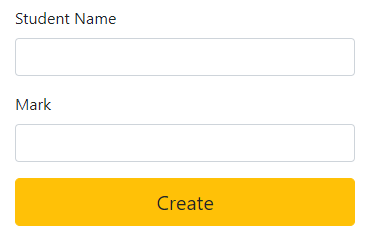
\includegraphics[scale = \picScale]{./images/lecturerUpdateMarks.png}}
	\vspace{-0.2cm}
	\caption{Update student marks page}
	\label{lecturerUpdateMarks}
\endminipage
\end{figure}



\subsection{Student Interface}
\begin{figure}[H]
\centering
\fbox{
\includegraphics[scale = 0.6]{./images/studentProfile.png}}
\caption{Student profile page}
\label{studentProfile}
\end{figure}



\section{Back-end}

%\begin{figure}[H]
%\centering
%\includegraphics[scale = 0.35]{./images/motorSchem.png}
%\caption{(a) Electrical diagram of a DC motor. (b) Sketch of DC motor \cite{dorf}.}
%\label{motorSchem}
%\end{figure}


%\newcommand{\picScale}{0.4}
%\newcommand{\minipageWidth}{0.46\textwidth}
%
%\begin{figure}[H]
%\minipage[t]{\minipageWidth}
%	\centering
%	\fbox{\includegraphics[scale = \picScale]{./images/stepResponse.png}}
%	\vspace{-0.2cm}
%	\caption{Graph showing the DC motor's step response.}
%	\label{stepResponse}
%\endminipage\hfill
%\minipage[t]{\minipageWidth}
%	\centering
%	\fbox{\includegraphics[scale = \picScale]{./images/naturalResponse.png}}
%	\vspace{-0.2cm}
%	\caption{Graph showing the DC motor's natural response.}
%	\label{naturalResponse}
%\endminipage
%\end{figure}

\section{Conclusion}

\subsection{Strenghts}

\subsection{Flaws}

\subsection{Improvements}

\subsection{Techniques Learned}
\addcontentsline{toc}{section}{References}
\nocite{*} % include this when you want to have all your (Jabref) references shown. comment out if you want only the ones that are used in the document diplayed.
\bibliographystyle{IEEEtran}
\bibliography{./ref} % the path to your filename of your .bib library


\end{document}
